
% !TEX root = ../../phdthesis_tawatr.tex 
\renewcommand{\thisdir}{_content/reg1d_exam}
\renewcommand{\figdir}{\thisdir/_fig}

\section[Examination of theoretical definition]{Consistency examination of the theoretical model of regional mean 1D conductivity profile}\label{sect:reg1d_exam}

%% Introductory paragraph
%\begin{itemize}
%	\item 
	In analogy to the fact that the host layer Earth is absolutely unknown in reality, we proposed to compare the estimated model of the regional mean 1D conductivity profile with the theorectical model of the regional mean 1D conductivity profile instead of comparing it with the true layer Earth (e.g., the model in Figure \ref{fig:lyrearth_model}) in synthetic tests.
%	\item 
	In this section, we examined the consistency of the proposed theoretical model (Eqs. \ref{eq:regional_mean_linear} and \ref{eq:regional_mean_log}) and the estimated model of regional mean 1D conductivity profile with synthetic examples.
%\end{itemize}

%% ==== ==== Go to the content
In conducting MT surveys and other geophysical methods, 
a number of observations are made to sufficiently cover the target structure with the typical site spacing to resolve the smallest scale target.
%
This concept is analogous to the sampling theorem. 
%
To demonstrate the effect of the array size, in this consistency test, we test the array size that is larger than and comparable to the anomaly size at different locations.


% ==== ====
We used the 3D models and the array setup (25 MT stations within an area of \areakm{80}{80}) as used in Section \ref{sect:example_3d}. In this setup, the cluster is significantly larger than the anomaly.
We put the cluster in the three different locations: central, northwest and northeast positions (Figure \ref{fig:model3d_setting_pp1}). 
%
At the center, the array is concentric with the anomaly, while at the northeast and northwest locations, the arrays are, respectively, dominated by the 300 and 3 \Ohmm\ anomalies. In this case, three clusters contain the same portion of conductive and resistive anomalies.

%% ==== checkerborad, cluster 80 x 80
\begin{figure}[!t]
	\centering
	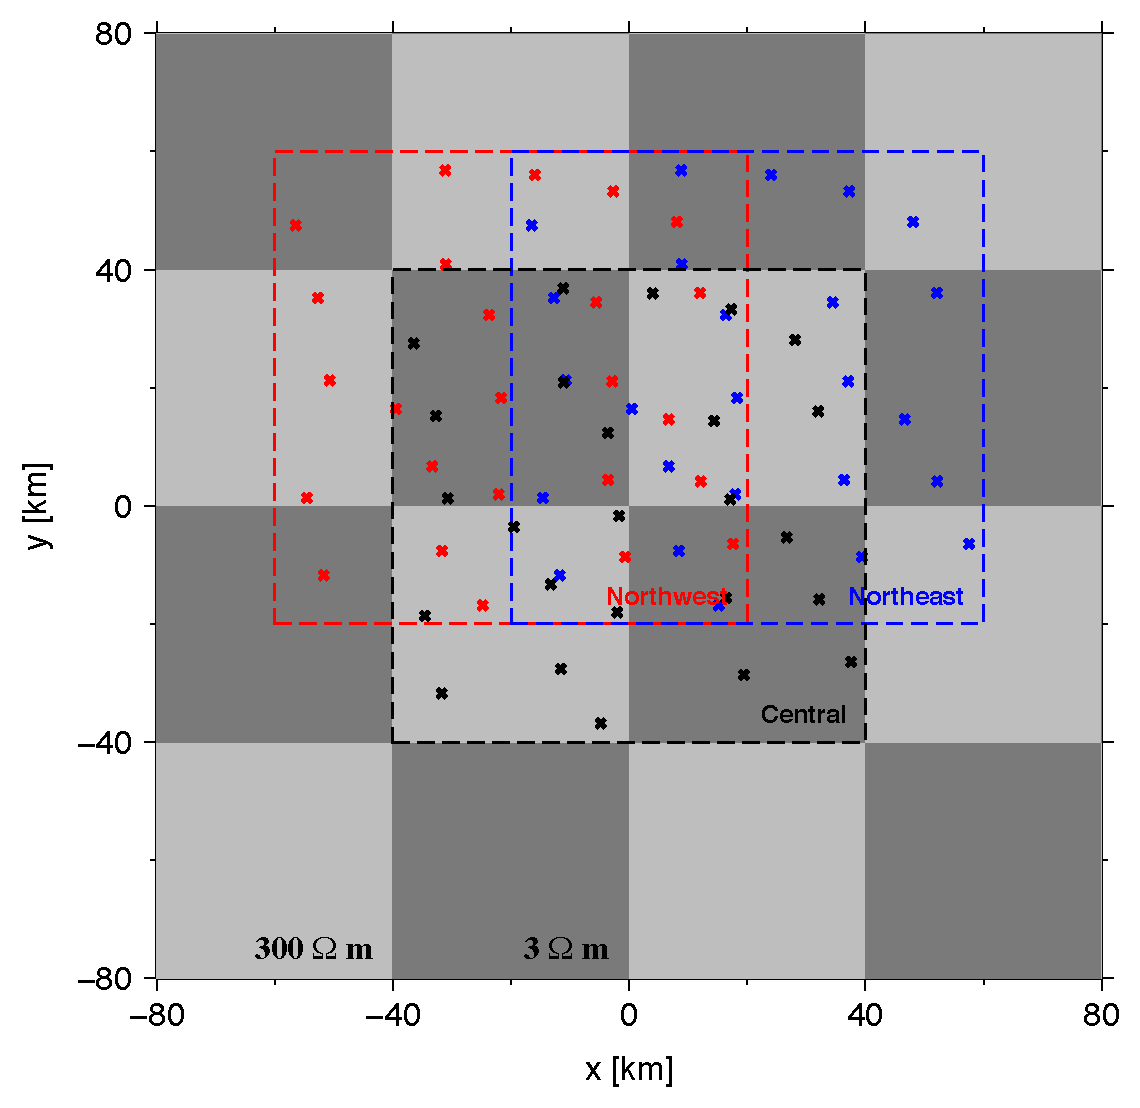
\includegraphics[width=\plotchkboardsize]{\figdir/m02a_chkboard12_h0a2a_s40k_pxpx_pp1.pdf}
	\caption[MT array, in which its size is comparable to the anomaly size, located at different position]{Checkerboard model with an anomaly size of {\areakm{40}{40}} and resistivities of 3 (dark gray) and 300 (light gray) {\Ohmm}. The checkerboard anomaly was embedded in the lower crust layer. Three arrays of 25 MT stations (crosses) each with a size of {\areakm{80}{80}}  (dashed frames) were placed at the central (black), northeast (blue), and northwest (red) positions.}
	\label{fig:model3d_setting_pp1}
\end{figure}
%% ==== checkerborad, cluster 80x80 results
\begin{figure}[!h]
	\centering
	\subfigure[]{
		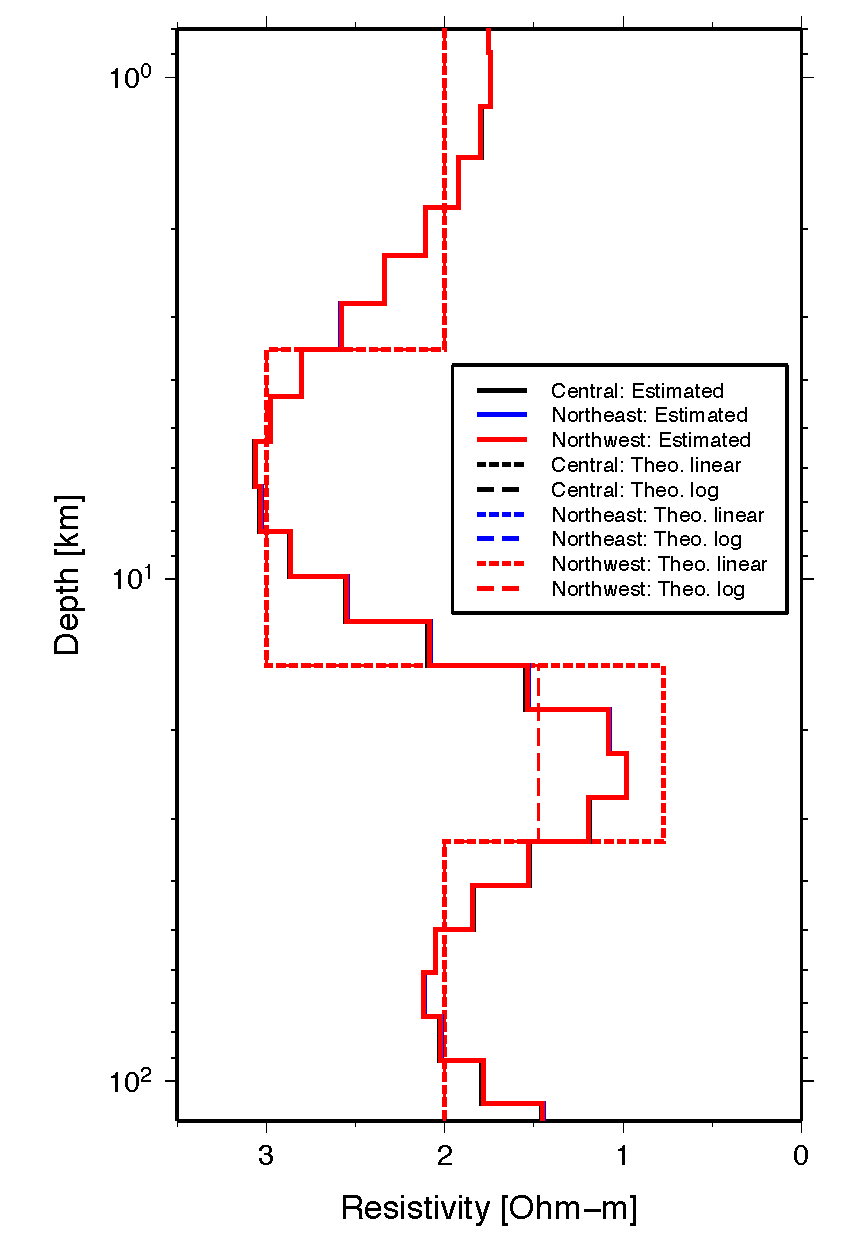
\includegraphics[scale=\plotinvmodelscale]{\figdir/m02a_lyr11a_chkboard12-h0a2a-d05a-t01a_chkboard1X_s40k_pxpx_pp1_d13a_ssq_r2.pdf}
		\label{fig:cb_resp_pxpx_pp1_model}
	}
	\subfigure[]{
		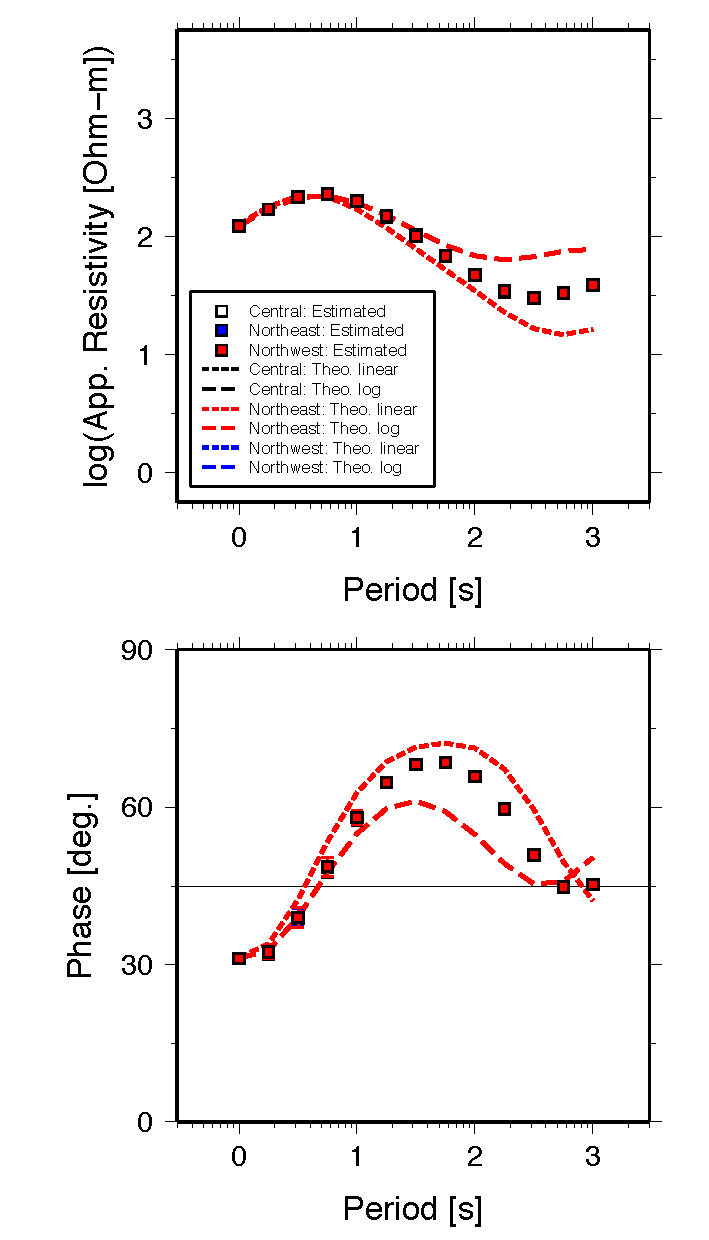
\includegraphics[scale=\plotmtrespscale]{\figdir/m02a_lyr11a_chkboard12-h0a2a-d05a-t01a_chkboard1X_s40k_pxpx_pp1_d13a_ssq_arsphs.pdf}
		\label{fig:cb_resp_pxpx_pp1_resp}
	}
	\caption[Theoretical and estimated model of regional mean 1D profile from large MT arrays]{(a) Theoretical (dashed lines) and estimated (solid lines) models of the mean 1D profiles obtained using the settings shown in Figure \ref{fig:model3d_setting_pp1}. (b) Corresponding MT responses from the theoretical (dashed line) and estimated (squares) models of the mean 1D profiles. The results obtained from different array locations are represented by lines and symbols of different colors.}
	\label{fig:cb_resp_pxpx_pp1}
\end{figure}

% ==== ====
The estimated models of the regional mean 1D conductivity profiles from these clusters were calculated from the average ssq impedance. Note that only the ssq impedance is used in this section, because the galvanic distortion is not of concern. 
%
The theoretical models of the regional mean 1D conductivity profile were calculated using the given definitions from the conductivity in the clusters (e.g., dashed frames in Figure \ref{fig:model3d_setting_pp1}), and
the MT responses from the theoretical models were then obtained using the analytic solution \citep{constable1987a}.

% ==== ==== Large array
%\redb{-- Large array --}

%\begin{itemize}
%	\item
When the arrays are larger than the anomaly, the arrays contain the comparable portions of the resistive and conductive heterogeneities, even though they are at different locations.
The estimated and theoretical models of the regional mean 1D conductivity profiles from different clusters are likely identical (Figure \ref{fig:cb_resp_pxpx_pp1}). 
In other words, the average approach is spatially independent for the large array. Hence, the average approach is a robust method to obtain the regional mean 1D conductivity profile.
%	\item
The smooth and step shapes of the estimated and theoretical models might be due to the smoothness constraint applied in the inversion.
%\end{itemize}




%% ==== ==== Small array.
%\redb{-- Small array --}

%\begin{itemize}
%	\item
Next, we demonstrate how array size affects the models of the regional mean 1D conductivity profile by decreasing the array size to \areakm{40}{40} (Figure \ref{fig:model3d_setting_pp0}), which is equal to the anomaly size. The cluster locations were kept the same as in the previous test.


%	\item
	In this case, the theoretical models from different cluster locations are totally different (Figure \ref{fig:cb_resp_pxpx_pp0_model}) because 
the clusters occupy different portions of resistive and conductive anomalies.
The northwest cluster covers only the underlying 3 {\Ohmm} anomaly, for example.
Note that when the array resides on the layered-Earth like structure, e.g., the cluster on the northwest and northeast positions, the theoretical models from the log and the linear average definition are the same (Figure \ref{fig:cb_resp_pxpx_pp0_model}). 
	%
	In constrast to the theoretical models, the estimated models of regional mean 1D profile remain spatially independent in this setup. This is because the inductive effect from the anomalies is indistinguishable from different array locations.
%	\item 
	It is expected that if the anomaly is significantly large or the cluster is very small, the estimation method would show the spatially dependent feature.
%\end{itemize}

%% ==== ==== Difference between the linear and log average
%\redb{-- Difference between the linear and log average --}

%\begin{itemize}
%	\item
	 As expected, using the logarithmic average definition (Eq. \ref{eq:regional_mean_log}) would give the less conductive structure (e.g., Figure \ref{fig:cb_resp_pxpx_pp1_model}). 
%	\item
	 Although, the theoretical models from the linear and log average definition are noticeably different (Figures \ref{fig:cb_resp_pxpx_pp1_model} and \ref{fig:cb_resp_pxpx_pp0_model}) when both conductive and resistive anomalied are contained in the array, they are both consistent with the estimated model. 
	Hence, both definitions are acceptable for calculating the theoretical model of the regional mean 1D conductivity profile.
%\end{itemize}

%% ==== ==== Describing the inconsistency
% \redb{-- Inconsistency --}
 
% \begin{itemize}
%	\item
	When the array is significantly larger than the anomaly, the estimation and the theoretical definition are rather consistent.
	But, when the array is comparable or smaller than the anomaly, the inconsistency is clearly observed, particularly, at the depth where the anomalies are embedded (Figure \ref{fig:cb_resp_pxpx_pp0}). 
%	\item 
	However, the inconsistency seems to be less evident when the cluster is located over the conductive anomaly (e.g., the northwest cluster), because of the nature of the electromagnetic induction that the conductive anomaly will produce significant inductive effect when compared to the resistive anomaly.
%	\item
	This inconsistency is a consequence of an inappropriate design of the observation array, e.g., the cluster is not sufficiently large to cover the anomaly. The tests also suggest that the estimation of the regional mean 1D profile would be reliable with a large size of array.
%\end{itemize}

%% ==== ==== Concluding paragraph
%\redb{-- Concluding paragraph --}

%\begin{itemize}	
%	\item 
	In general, the exact dimension of the target structure is unknown. One may be able to approximate its from other information such as geological background or past studies.
%	\item
	The observation array is then designed so as to cover the target structure.
%	\item 
	However, if the anomaly geometry is found to be comparable to the size of the array then the resulting conductivity image may be affected by the array location. One suggestion is to increase the array size by adding additional MT stations in order to get the reliable results.
%\end{itemize}

%\red{This synthetic example gives the instructive suggestion for the design of observation array according to the target structure.}

%% ==== ==== Figure



%% ==== checkerborad, cluster 40x40 
\begin{figure}[!h]
	\centering
	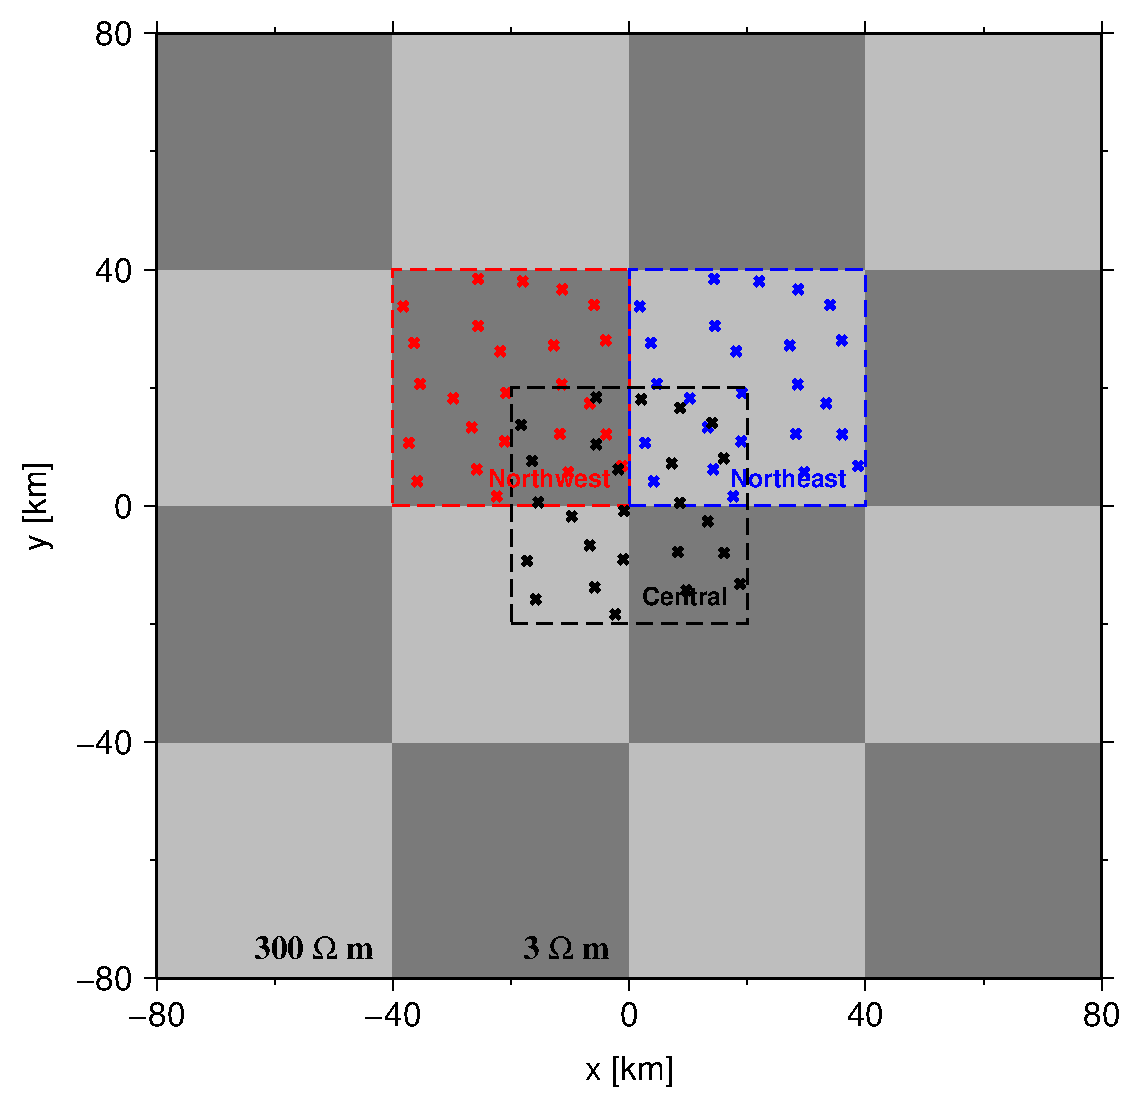
\includegraphics[width=\plotchkboardsize]{\figdir/m02a_chkboard12_h0a2a_s40k_pxpx_pp0.pdf}
	\caption[Same as Figure \ref{fig:cb_resp_pxpx_pp1} for small arrays]{Same as Figure \ref{fig:cb_resp_pxpx_pp1} for an array size of \areakm{40}{40}.}
	\label{fig:model3d_setting_pp0}
\end{figure}

%% ==== checkerborad, cluster 40x40 results
\begin{figure}[t]
	\centering
	\subfigure[]{
		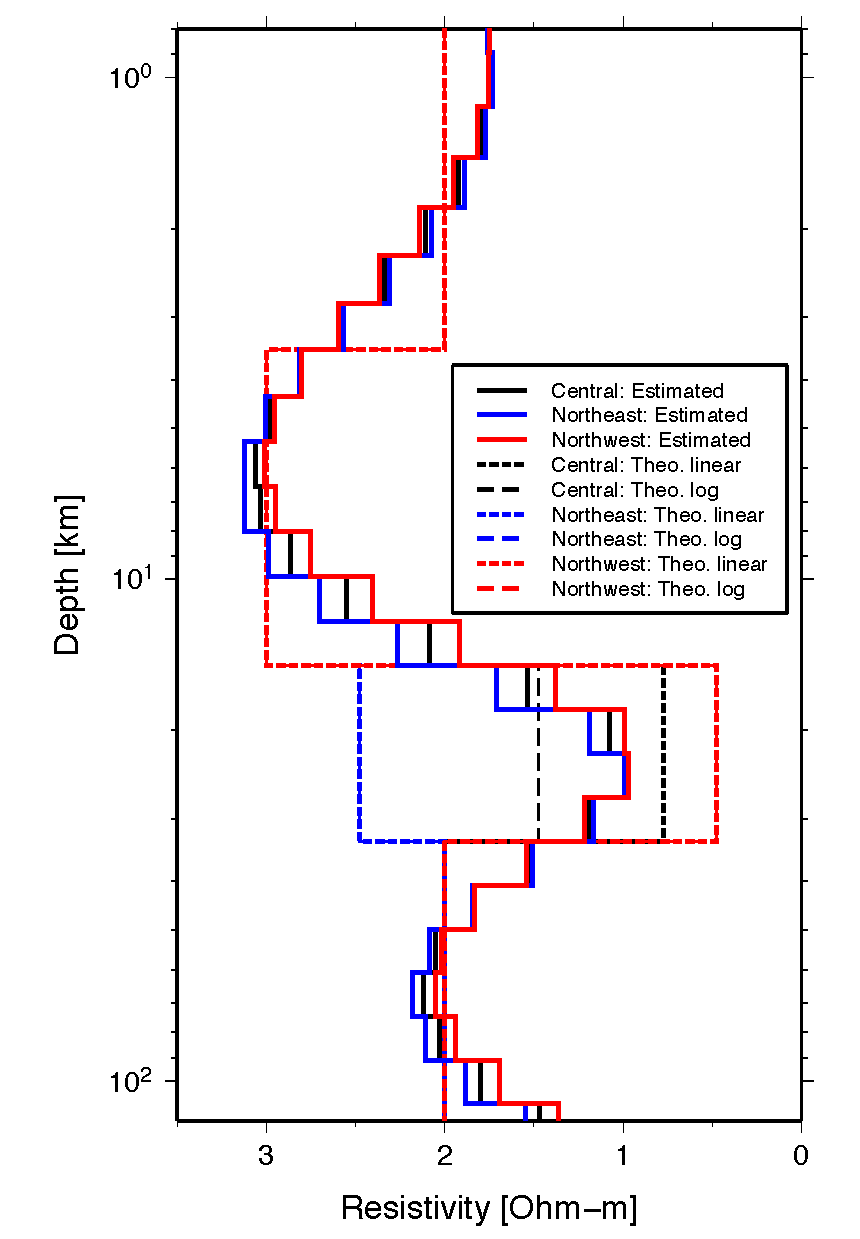
\includegraphics[scale=\plotinvmodelscale]{\figdir/m02a_lyr11a_chkboard12-h0a2a-d05a-t01a_chkboard1X_s40k_pxpx_pp0_d13a_ssq_r2.pdf}
		\label{fig:cb_resp_pxpx_pp0_model}
	}
	\subfigure[]{
		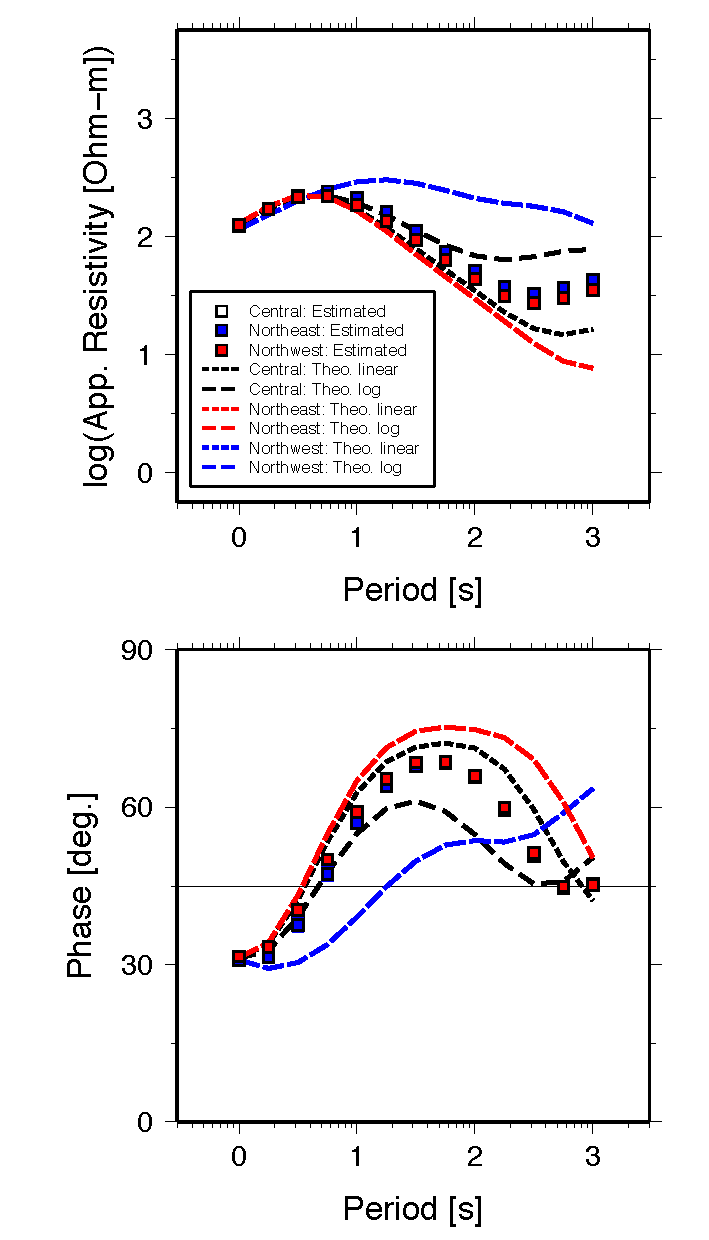
\includegraphics[scale=\plotmtrespscale]{\figdir/m02a_lyr11a_chkboard12-h0a2a-d05a-t01a_chkboard1X_s40k_pxpx_pp0_d13a_ssq_arsphs.pdf}
		\label{fig:cb_resp_pxpx_pp0_resp}
	}
	\caption{Same as Figure \ref{fig:cb_resp_pxpx_pp1} for the settings shown in Figure \ref{fig:model3d_setting_pp0}.}
	\label{fig:cb_resp_pxpx_pp0}
\end{figure}
